\chapter{Oprogramowanie Sterujące}
\label{cha:Software}
\section{Firmware - Oprogramowanie mikrokontrolera}
Firmware można podzielić na dwie części. Oprogramowanie open-source płytki sterownika do silników szczotkowych oraz właściwy skaner. Wspomniane oprogramowanie płytki sterownika wpiera już kontrolę prędkości obracania się pojedynczego silnika, oraz włączanie i wyłączanie silnika. Dodatkowo wspiera komunikację za pomocą komend powłoki (shell commands) transmitowanych po USB oraz Bluetooth LE. Na potrzeby tego projektu należy je rozwinąć o dodatkowy tryb kontroli - kontrola pozycji. Posiadając kontroler do silników szczotkowych zdolny do osiągnięcia zadanej pozycji, będzie możliwe napisanie wyższej warstwy abstrakcji - skanera, przyjmującego kolejne pozycje zgodnie ze zdefiniowaną macierzą punktów. Dodatkową zaletą podziału oprogramowania mikrokontrolera na dwie warstwy jest rozwój uniwersalnego sterownika do silników o kontrolę pozycji, który będzie można wykorzystać w wielu kolejnych projektach. Architektura ta przedstawiona jest na schemacie \ref{img:general_class_diag}.

\begin{figure}[h!] 
\centering 
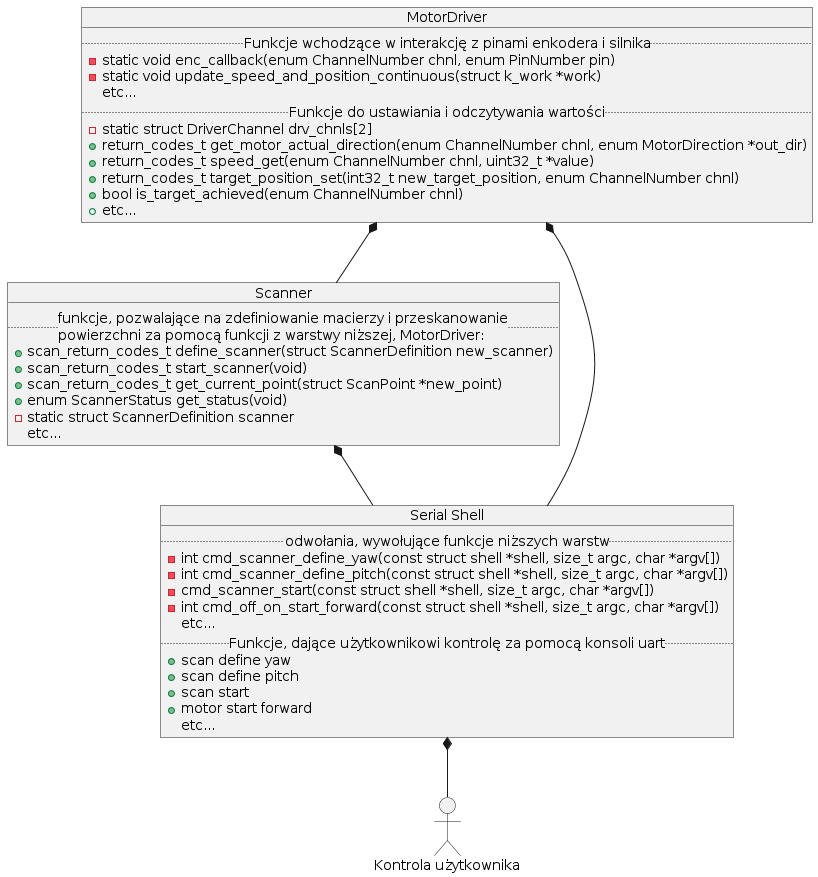
\includegraphics[width=0.9\textwidth]{img/ClassDiagGenUML.png}
\caption{Uogólniony schemat architektury oprogramowania}
\label{img:general_class_diag}
\end{figure}

Całość oprogramowania na mikrokontroler jest napisana w języku C, używając bibliotek HAL (Hardware Abstraction Layer) środowiska RTOS (Real Time Operataing System) Zephyr. Jest to zestaw open-sourcowych bibliotek, wspieranych między innymi przez firmę Nordic Semiconductors, która jest producentem procesora nRF52840. Głównymi zaletami Zephyra jest mały rozmiar budowanego kodu, wsparcie dla procesorów wielu producentów oraz licencja Apache 2.0. W architekturze Zephyra wsparcie różnych procesorów jest rozwiązane za pomocą Devicetree. Jest to oddzielny opis architektury wewnętrznej mikrokontrolera, jak piny, rejestry czy peryferia, ale też dodatkowych komponentów znajdujących się na płytce. Pozwala to na łatwe przenoszenie kodu między różnymi procesorami. \cite{Zephyr_docs}

Wspomniana na diagramie \ref{img:general_class_diag} architektura mocno opiera się o API programistyczne (\textbf{Application Programming Interface}; Interfejs Programowania Aplikacji). Jest to sposób, w jaki dwa programy albo komponenty oprogramowania wchodzą ze sobą w interakcję. \cite{api} Czyli upraszczając, w przypadku tego projektu jest to pewien zestaw publicznych funkcji i zmiennych, które w zaprojektowanej przez programistę bibliotece stanowią interfejs, za pomocą którego można z tą biblioteką wchodzić w interakcję. Wspomniane są także warstwy abstrakcji. Jako warstwę abstrakcji można uznać pewien zamknięty fragment kodu implementujący konkretną funkcjonalność, pozwalający na proste ponowne użycie tego fragmentu w kolejnym projekcie oraz zamykający skomplikowany kod za prostym interfejsem, np. poprzez zastosowanie pewnego API. \cite{abstraction_layer} Poprawne zaimplementowanie kodu, który stosuje zrozumiałe API oraz utrzymuje poprawny podział na warstwy abstrakcji, to pierwszy krok do zachowania zasad z grupy SOLID. Jest to mnemoniczny akronim pod którym kryje się 5 zasad tworzenia oprogramowania które jest skalowalne, zrozumiałe oraz łatwe w utrzymaniu. \cite{solid}

\subsection{Skalowalne rozwiązanie wielokanałowe}
\label{cha:second_channel}
Na potrzeby kontroli pozycji dookoła dwóch osi, należało zrefaktoryzować obecną kontrolę prędkości oraz zaimplementować nową kontrolę pozycji w sposób skalowalny. W celu osiągnięcia tego założenia, powstała struktura, opisująca pojedynczy kanał kontrolera. Jej interfejs przedstawiony jest na \ref{img:driver_channel_diag}.

\begin{figure}[h!] 
\centering 
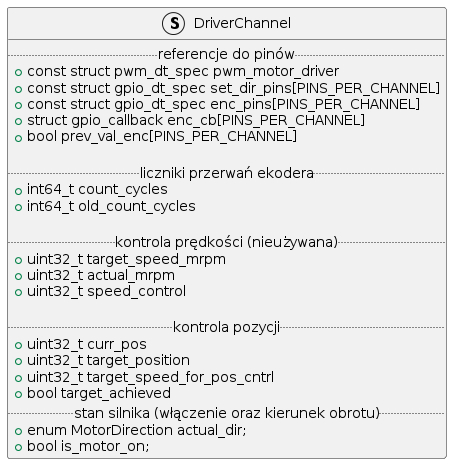
\includegraphics[width=0.5\textwidth]{img/DriverChannelUML.png}
\caption{Interfejs struktury opisującej kanał sterownika.}
\label{img:driver_channel_diag}
\end{figure}

Następnie została utworzona skalowalna tablica kanałów \texttt{drv\_chnls} typu \texttt{static struct DriverChannel}. W przypadku tego projektu ma ona zaledwie 2 elementy, ale może być skalowana dowolnie, w zależnie od możliwości sprzętowych. Opisywana lista struktur zaimplementowana jest wewnątrz pliku driver.c (który zawiera implementację sterownika) i jedynie funkcje z tego pliku mają do niej dostęp.

Każda funkcja ze wspominanego pliku przyjmuje numer kanału typu \texttt{enum ChannelNumber}. Wewnątrz poszczególnych funkcji numer kanału stanowi odniesienie do odpowiedniego elementu wcześniej opisywanej tablicy. Jest to dobry przykład architektury open-closed (litera O ze skrótu SOLID), gdzie programista daje użytkownikowi jedynie zestaw funkcji, tutaj zdefiniowanych w pliku driver.h, za pomocą których użytkownik (programista używający API) odnosi się do wewnętrznej, zamkniętej implementacji, która może ulec zmianie, bez wpływania na interfejs użytkownika.

\subsection{Kontrola pozycji silnika szczotkowego}
\label{cha:pos_control}
\subsubsection{Przerwanie od pinów enkodera}
Podstawą precyzyjnego wyznaczania pozycji silnika szczotkowego jest poprawnie działające przerwanie od enkodera. Enkoder pojedynczego silnika składa się z dwóch pinów, podczas normalnej pracy - obracania się ze stałą prędkością w jednym kierunku - na piny te podawana jest fala prostokątna, przesunięta w fazie o $\frac{1}{4}$ okresu. Przesunięcie to pozwala na wyznaczenie kierunku ruchu silnika. Dla pinu 1, jeżeli wartości pinów są różne, to silnik kręci się do przodu, jeżeli takie same, to w przeciwnym kierunku. W przerwaniu od pinu 2 jest na odwrót - dla wartości takich samych obrót następuje do przodu. Dalej w zależności od kierunku, następuje inkrementacja bądź dekrementacja licznika. \cite{rotary_encoder_tutorial} Funkcja, odpowiedzialna za zliczanie przerwań, przedstawiona jest na schemacie \ref{img:encoder_callback}. Jest to przepływ logiki zaprezentowany jedynie dla jednego kanału. Cały ten proces wykonywany jest osobno dla obu kanałów, a dodatkowo na \ref{img:driver_channel_diag} widać, że faktycznie, \texttt{count\_cycles} jest zdefiniowany osobno, dla obu kanałów.

\begin{figure}[h!] 
\centering 
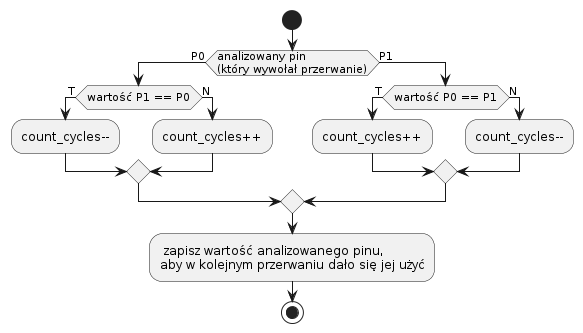
\includegraphics[width=0.8\textwidth]{img/PinInterruptUML.png}
\caption{Przepływ logiki przerwania od pinu enkodera na pojedynczym kanale.}
\label{img:encoder_callback}
\end{figure}

\subsubsection{Przerwanie od zegara}
Przerwanie od enkodera może być wywoływane bardzo często - przy maksymalnej prędkości użytego silnika ponad 10 razy na milisekundę ($\frac{RPM \cdot CPR}{60 \cdot 1000} = \frac{67 \cdot 9600}{60 * 1000} = 10.72 $), a należy pamiętać że jest to najwolniejszy silnik z tej linii produktu. Biorąc pod uwagę, że efektem tej pracy ma być uniwersalny sterownik do silników, trzeba uwzględnić także szybsze jednostki. Z tego powodu nie można umieszczać w tym przerwaniu zbyt zaawansowanego kodu, jedynie podstawowe obliczenia, jak inkrementacja odpowiedniej zmiennej. Właściwe obliczenia pozycji, a także prędkości, której kontrolę także trzeba utrzymać aby zachować wsteczną kompatybilność, są realizowane w osobnym przerwaniu, od zegara, które jest wywoływane co $20ms$. Czas tego przerwania jest zmienną czasu kompilacji i może być swobodnie dostosowywany w pliku \texttt{prj.conf}, w zależności od potrzeb projektowych. Oczywiście im ten czas będzie mniejszy, tym kontrola powinna być precyzyjniejsza, ponieważ przerwanie obliczające obecną pozycję, prędkość i kierunek ruchu będzie wywoływane częściej. Ale też należy pamiętać, że im częściej przerwanie to będzie wywoływane, tym większe ryzyko, że kolejne przerwanie rozpocznie się, zanim poprzednie się zakończy, co przy obecnej implementacji spowoduje, że kolejka zadań (task work queue) zapcha się i procesor zawiesi się. Jest to problem, który da się jedynie rozwiązać zastosowaniem mocniejszego (na przykład wielowątkowego) procesora lub zmniejszeniem częstotliwości przerwań.

Przerwanie od zegara jest najważniejszą funkcją całego sterownika. To w niej dzieją się całe obliczenia. Na potrzeby kontroli pozycji powstały dwa duże, istotne, fragmenty tej funkcji. Pierwszym z nich jest odczytywanie obecnej pozycji, przedstawione na schemacie \ref{img:pos_calc_UML}. Jest to wykonywane zawsze, w każdym cyklu przerwania, dla każdego kanału. Drugim fragmentem jest sama kontrola pozycji, przedstawiona na schemacie \ref{img:pos_settin_UML}. Kod ten jest zależny od wartości stałych kompilacyjnych. Zostanie wywołany tylko przy ich odpowiednich wartościach, które na potrzeby tego projektu zostały ustawione w kombinacji - kontrola pozycji włączona, prędkości wyłączona. Rozróżnienie takie jest wymagane aby zachować wsteczną kompatybilność z poprzednimi projektami.

\subsubsection{Obliczanie pozycji}
\label{cha:calc_pos}

\begin{figure}[h!] 
\centering 
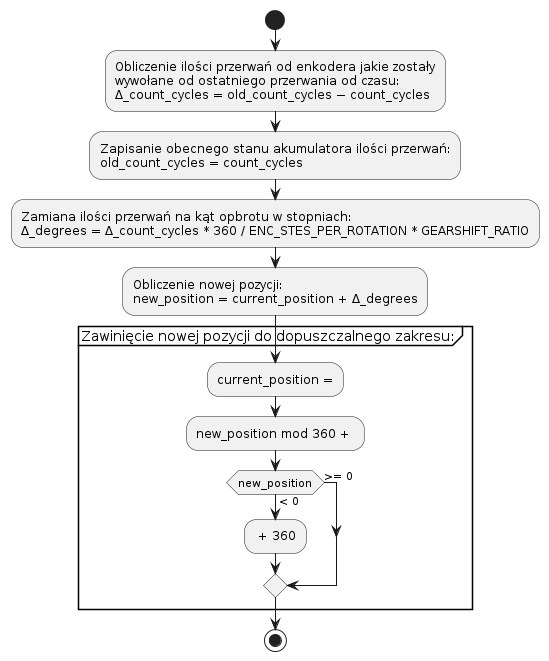
\includegraphics[width=0.8\textwidth]{img/CalcNewPos.png}
\caption{Diagram obliczania obecnej pozycji dla jednego kanału.}
\label{img:pos_calc_UML}
\end{figure}

Obliczanie pozycji odbywa się w kilku krokach. Pierwszy krok to obliczenie przyrostu ilości przerwań enkodera od ostatniego wywołania przerwania od czasu. Znając obecną wartość akumulatora \texttt{count\_cycles}, oraz jego wartość która została zapisana podczas poprzedniego cyklu, można obliczyć różnicę $\Delta_{count\_cycles} = old\_count\_cycles - count\_cycles$. Następnie po tych obliczeniach obecna wartość \texttt{count\_cycles} jest zapisywana dla zmiennej \texttt{old\_count\_cycles}, na potrzeby kolejnego przerwania od czasu. Kolejny krok, to skalowanie, zamiana jednostek - przeliczenie $\Delta_{count\_cycles}$, na stopnie. Odbywa się to za pomocą wzoru \ref{eq:cycles_to_deg}. Wzór ten zawiera zmienne \texttt{ENC\_STEPS\_PER\_ROTATION} oraz \texttt{GEARSHIFT\_RATIO}, które są zmiennymi czasu kompilacji zdefiniowanymi w pliku Kconfig.motor, i ich wartości powinny odpowiadać wartościom odczytanym z dokumentacji użytych silników. Dla silnika Pololu 2828 wynoszą odpowiednio:
\vspace{-\topsep}
\begin{itemize}
    \item \texttt{ENC\_STEPS\_PER\_ROTATION = 64},
    \item \texttt{GEARSHIFT\_RATIO = 150},
\end{itemize}
\vspace{-\topsep}

\begin{equation}
\label{eq:cycles_to_deg}
    \Delta_{degrees} = \frac{\Delta_{count\_cycles} \cdot 360^{\circ}}
		  {ENC\_STEPS\_PER\_ROTATION \cdot GEARSHIFT\_RATIO}
\end{equation}

Kolejny krok jest bardzo prosty, polega na dodaniu obliczonej $\Delta_{degrees}$ do akumulatora \texttt{current\_position}, przechowującego ostatnią faktyczną pozycję silnika. Tutaj należy pamiętać, że w zależności od kierunku obrotu silnika wartość $\Delta_{degrees}$ może być ujemna. Może to spowodować, że \texttt{current\_position} przyjmie także wartość ujemną. Nie jest to pożądana sytuacja, jako że idea stojąca za wspomnianą zmienną jest inna - powinna ona przechowywać wartość z zakresu $0 - 360^{\circ}$. Dlatego też nie następuje od razu przypisanie nowej wartości do tej zmiennej. Obecna wartość zmiennej \texttt{current\_position} jest tymczasowo zamieniana z typu \texttt{unsigned int} na \texttt{int}, co pozwala na użycie jej ze znakiem. Następnie nowa wartość jest przenoszona do zakresu $0 - 360^{\circ}$ zgodnie ze wzorem \ref{eq:wrap_current_deg_pos}, aby na samym końcu nadpisać starą wartość zmiennej.

\begin{equation}
\label{eq:wrap_current_deg_pos}
    current\_position = ( new\_position \mod 360^{\circ} ) + 
    \begin{cases}
      360^{\circ} & \text{jeżeli } new\_position < 0\\
      0 & \text{w przeciwnym wypadku}\\
    \end{cases}
\end{equation}

Cały algorytm, opisywany w tym rozdziale, został zamknięty w trzech makrach, co pozwala na jego zapis w zaledwie jednej linijce kodu i bardzo szybki czas wykonania. W celu lepszej wizualizacji, został on także zaprezentowany w formie diagramu \ref{img:pos_calc_UML}. Rysunek ten przedstawia algorytm dla jednego kanału. Makra odpowiedzialne za wspomniane obliczenia przyjmują jako argument także numer kanału i odnoszą się do odpowiednich zmiennych, zdefiniowanych jako część danego kanału.



\subsubsection{Ruch do pozycji docelowej}
Ruch do pozycji docelowej jest bardziej skomplikowanym spośród dwóch algorytmów wykonywanych w ramach cyklicznego przerwania od czasu. W pierwszej kolejności należy obliczyć deltę, różnicę między punktem obecnym a punktem docelowym. Wartość oraz znak tej różnicy będą w pierwszej kolejności mówiły o kierunku, w którym powinien zacząć obracać się silnik. Jest to widoczne w pierwszej części schematu przedstawionego na rys. \ref{img:pos_settin_UML}. Widać, że wartość absolutna tej różnicy wpływa na to, od której strony wał dotrze do punktu docelowego. Jeżeli jest większa od $180^{\circ}$, to silnik dotrze do punktu "od tyłu", natomiast jeżeli jest mniejsza, to dotrze do punktu "od przodu". Natomiast znak wartości tej różnicy - część schematu sprawdzająca, czy zmienna \texttt{position\_delta} jest ujemna czy dodatnia - odpowiada za ustalenie po której stronie obecnej pozycji wału silnika znajduje się "przód"\ punktu, a po której "tył"\ punktu.

\begin{figure}[h!] 
\centering 
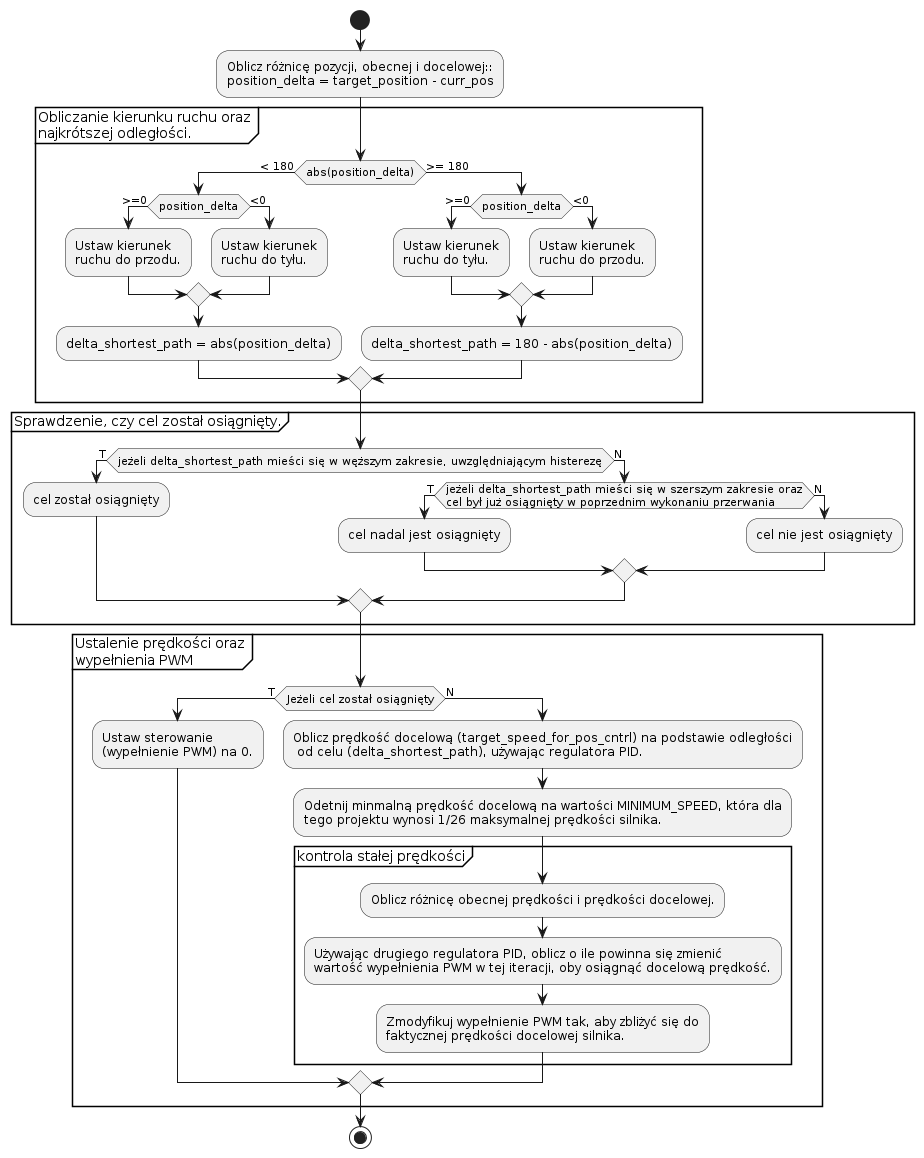
\includegraphics[width=\textwidth]{img/PosSettingUML.png}
\caption{Ruch do pozycji docelowej.}
\label{img:pos_settin_UML}
\end{figure}

Kolejnym fragmentem diagramu \ref{img:pos_settin_UML} jest sprawdzenie, czy wał silnika osiągnął zadaną pozycję docelową. Z powodu problemu, jaki pojawił się w czasie testów urządzenia, musi odbywać się to w dwóch krokach. Po osiągnięciu pozycji, napięcie na przekładni połączone z masą poruszanego obiektu powodowały, że wał silnika cofał się o kilka setnych stopnia. W zależności od jego dokładnej pozycji, mogło to spowodować opuszczenie dopuszczalnego zakresu. Dlatego też wymusiło to dodanie swego rodzaju histerezy. I to właśnie wspomniana histereza jest sprawdzana w pierwszej kolejności. Ogranicza ona dopuszczalny zakres kątów o pewien procent, co wymusza na sterowniku precyzyjniejszą kontrolę właśnie o ten procent. Natomiast, aby wyeliminować opisywany powyżej problem, główny dopuszczalny obszar jest nieco szerszy. Jeżeli w poprzednim wykonaniu przerwania osiągnięty już został obszar węższy, uwzględniający histerezę, to w kolejnym wykonaniu dopuszczalny obszar jest odrobinę większy. Eliminuje to ryzyko, że mikro ruchy na granicy obszaru wymuszą ponowny ruch wibrometru i jego ponowną próbę osiągnięcia wymaganego zakresu. Obszary te są zdefiniowane jako zmienne kompilacyjne w pliku prj.conf i wynoszą:
\vspace{-\topsep}
\begin{itemize}
    \item \texttt{POS\_CONTROL\_PRECISION\_MODIFIER = 480}, co daje obszar $\pm 0.75^{\circ}$
    \item \texttt{POS\_CONTROL\_HISTERESIS\_PERCENTAGE = 40\%}, co daje obszar $\pm 0.3^{\circ}$
\end{itemize}

Ostatnim, najbardziej istotnym, fragmentem ustalania pozycji jest sam regulator PID (\textbf{Proportional–integral–derivative controller}, regulator proporcjonalno-całkująco-różniczkujący), a raczej tandem dwóch regulatorów PID. W pierwszej kolejności na podstawie wcześniej obliczonej, najkrótszej odległości od celu ustalona zostaje prędkość, z jaką powinien kręcić się silnik. Prędkość ta jest proporcjonalna do odległości, zgodnie z zasadą działania człona P regulatora. Jest ona także odcinana na minimalnej ustalonej wartości prędkości, aby wyeliminować problemy pojawiające się przy próbie wymuszenia bardzo małych prędkości silnika szczotkowego. W tym miejscy należy zwrócić uwagę, że wyjściem tego regulatora jest prędkość. Sterowaniem całego układu jest natomiast wypełnienie PWM, od którego prędkość jest zależna. Jednakże, zwłaszcza przy zastosowaniu znacznych obciążeń, ta zależność nie będzie liniowa. Dlatego też został zaimplementowany drugi regulator PID, który na wejście otrzymuje wcześniej obliczoną prędkość docelową oraz faktyczną obecną prędkość silnika. Natomiast jego wyjściem jest przyrost wartości wypełnienia,  wymagany aby otrzymać faktyczną docelową prędkość silnika. Tak zmodyfikowana wartość wypełnienia PWM jest podawana na układ sterownika Toshiba.

Wspomniany wyżej regulator PID został zaimplementowany zgodnie z uproszczonym wzorem \ref{eq:pid_equation}, gdzie $\Delta_{akumulator}$ oznacza sumę wszystkich poprzednich wartości $\Delta$, natomiast $\Delta_{poprzednia\_wartość}$ oznacza wartość $\Delta$ z poprzedniego wykonania przerwania. $\Delta$ natomiast to tak zwany błąd, czyli różnica między wartością (czy prędkości, czy pozycji) obecną, a docelową. Parametry $Kp$, $Ki$ oraz $Kd$ to nastawy regulatora, dobierane indywidualnie na potrzeby projektu.

\begin{equation} \label{eq:pid_equation}
    sterowanie = Kp \cdot \Delta + Ki \cdot \Delta_{akumulator} + Kd \cdot \Delta_{poprzednia\_wartosc}
\end{equation}

Nastawy obu regulatorów PID zostały dobrane empirycznie, tak aby sprawdzały się przy małych prędkościach obrotu, jeden komplet dla obu kanałów. Podczas dostrajania został użyty jedynie człon P, a wartości $Ki$ oraz $Kd$ zostały ustawione na $0$. Użycie tych członów okazało się nie być potrzebne do poprawnego ruchu wibrometru. Ostatecznie wartości $Kp$ dla dwóch kolejnych regulatorów zostały kolejno ustawione na:
\vspace{-\topsep}
\begin{itemize}
    \item $Kp_{kontroli\_pozycji} = 2\frac{1}{2}$
    \item $Kp_{kontroli\_predkości} = \frac{1}{2}$
\end{itemize}

W tym miejscu, tak samo jak w przypadku rozdziału \ref{cha:calc_pos}, należy pamiętać, że algorytm przedstawiony na schemacie \ref{img:pos_settin_UML} ilustruje jedynie przepływ logiki dla jednego kanału. W ramach opisywanego przerwania od czasu, jest on wykonywany dwa razy, osobno dla obu kanałów, a opisywane zmienne stanowią część listy struktur opisywanej w rozdziale \ref{cha:second_channel} oraz są przedstawione na diagramie \ref{img:driver_channel_diag}.

\subsection{Algorytm skanujący}
\label{cha:scan_alg}
Algorytm korzysta z API, będącego interfejsem niższej warstwy oprogramowania, opisywanej w rozdziale \ref{cha:pos_control}. API udostępnia interfejsy pozwalające kontrolować pozycję silników na poszczególnych kanałach i jest zaprojektowane w taki sposób, aby algorytmy stojące za kontrolą pozycji nie miały wpływu na pracę programisty tworzącego warstwę skanera.

Cały proces skanowania zaczyna się od zdefiniowania oraz przygotowania skanera, a odpowiedzialna jest za to funkcja \texttt{define\_scanner}. Funkcja ta przygotowuje kontroler poprzez wyłączenie silników (tylko jeżeli użytkownik zostawił je włączone po poprzedniej operacji) oraz ustawienie odpowiedniego trybu pracy - kontroli pozycji. Następnie ustawia wewnętrzną instancję skanera, znajdującego się pod zmienną \texttt{struct ScannerDefinition scanner} na definicję skanera przekazaną jako argument do funkcji. Definicja ta jest typu \texttt{struct ScannerDefinition}, który opisuje wszystkie parametry definiowanego skanera. Struktura ta jest przedstawiona na schemacie \ref{img:scanner_def_uml}.

\begin{figure}[h!] 
\centering 
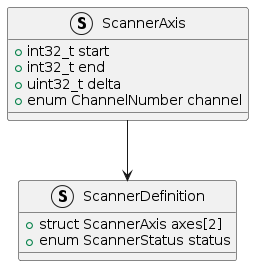
\includegraphics[width=0.4\textwidth]{img/ScannerDefUML.png}
\caption{Struktura opisująca parametry skanera.}
\label{img:scanner_def_uml}
\end{figure}

Na schemacie \ref{img:scanner_def_uml} widać także wzmiankę o statusie skanera. Także znaczna większość funkcji, włącznie z definiowaniem skanera, zawiera sprawdzenia statusów. Koncept maszyny stanów statusów skanera jest dokładnie wyjaśniony w rozdziale \ref{cha:state_machine}.


Kolejnym krokiem algorytmu jest startowanie skanera. Start, poza standardowymi sprawdzeniami statusu, ustawia obecny cel (zmienna \texttt{target}) i przekazuje ten cel warstwę niżej, poprzez API sterownika do silników, za pomocą funkcji \texttt{target\_position\_set}. Odbywa się też wtedy start zegara \texttt{wait\_for\_point\_timer}, którego przerwanie ma za zadanie sprawdzać, czy punkt zadany został już osiągnięty. Logika tejże funkcji przedstawiona jest na \ref{img:wait_for_point_handler}.

\begin{figure}[h!] 
\centering 
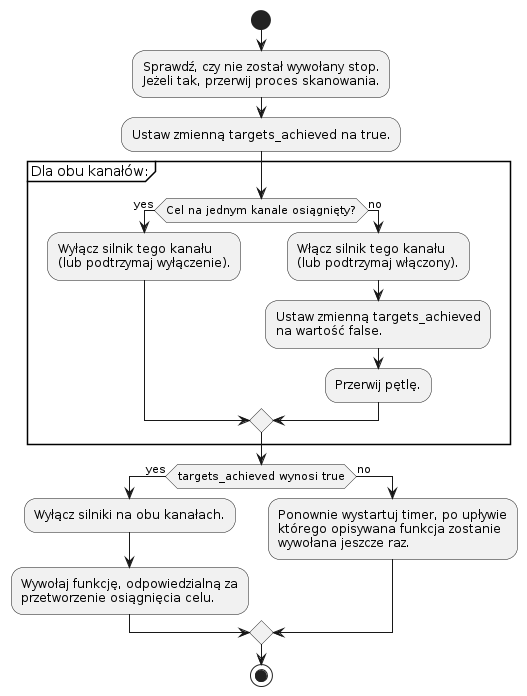
\includegraphics[width=0.7\textwidth]{img/WaitForPointUML.png}
\caption{Przepływ logiki funkcji \texttt{wait\_for\_point\_handler()}.}
\label{img:wait_for_point_handler}
\end{figure}

Diagram \ref{img:wait_for_point_handler} pokazuje logikę, którą można opisać jako utrzymywanie jednego kanału włączonego, dopóki cel nie jest osiągnięty, a następnie załączenie drugiego kanału. Natomiast pod koniec wspomniana jest funkcja, która przetwarza osiągnięcie celu przez oba kanały (na obu osiach urządzenia). Funkcja ta, jest głównym miejscem całego algorytmu, gdzie podejmowane są decyzje oraz wykonywane wszystkie istotne obliczenia. Przepływ logiki tejże funkcji przedstawiony jest na diagramie \ref{img:point_achieved_handler}.

\begin{figure}[h!] 
\centering 
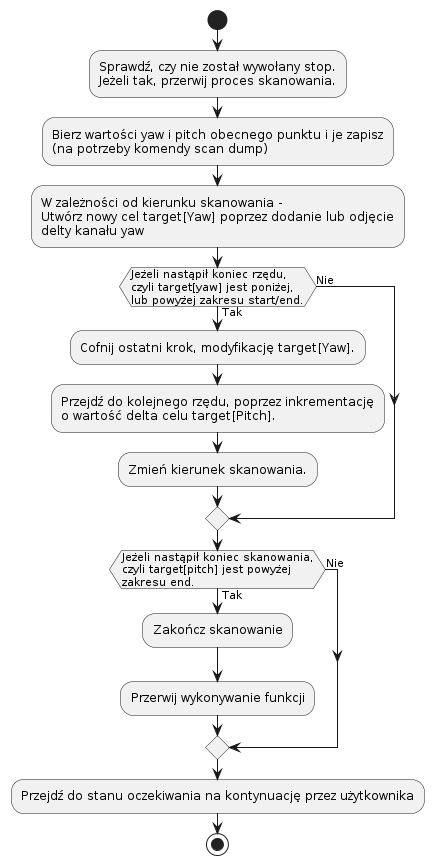
\includegraphics[width=0.6\textwidth]{img/PointAchievedUML.png}
\caption{Przepływ logiki funkcji \texttt{point\_achieved\_handler()}.}
\label{img:point_achieved_handler}
\end{figure}

Patrząc na diagram \ref{img:point_achieved_handler} można wywnioskować, że funkcja \texttt{point\_achieved\_handler()} odpowiedzialna jest za podjęcie decyzji, jakie mają być wartości kolejnego punktu, do którego będzie zmierzać urządzenie. Schemat jej działania można uprościć do opisu: Wpierw następuje przeskanowanie pierwszego rzędu, zwiększając cel na osi yaw z każdym wywołaniem tej funkcji. Następnie, jeżeli kolejny punkt miałby przekroczyć wartość zdefiniowaną jako \texttt{yaw\_end} funkcja ta zmienia rząd, oraz kierunek ruchu silnika umieszczonego w osi yaw (pionowej, z). Jeżeli zwiększenie rzędu miałoby spowodować wartość na osi pitch większą niż \texttt{pitch\_end} - następuje zakończ skanowanie.

Funkcja, jak wskazano na diagramie \ref{img:point_achieved_handler} kończy się oczekiwaniem na reakcję użytkownika. Reakcja następuje po wywołaniu funkcji \texttt{move\_to\_next\_point()}. Działa ona bardzo podobnie do startu, z pominięciem ustawiania nowego celu, cel został już ustawiony. Podaje ona jedynie te cele do funkcji \texttt{target\_position\_set} i startuje zegar \texttt{wait\_for\_point\_timer}. W tym momencie następuje powrót do odwołania od tego zegara opisanego w \ref{img:wait_for_point_handler}.

\subsection{Maszyna stanów urządzenia}
\label{cha:state_machine}
\begin{figure}[h!] 
\centering 
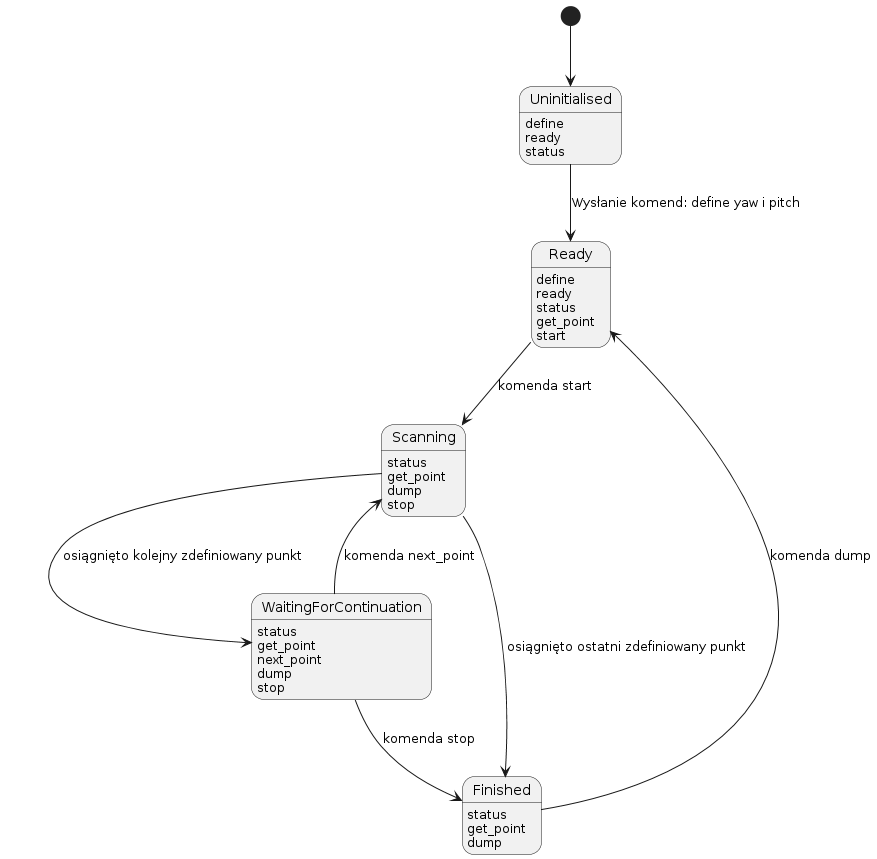
\includegraphics[width=\textwidth]{img/StatesUML.png}
\caption{Maszyna stanów urządzenia.}
\label{img:states_uml}
\end{figure}
Aby zabezpieczyć urządzenie przed wykonywaniem niedozwolonych operacji, oraz potencjalnym uszkodzeniem, powstała maszyna stanów, a każda funkcja jest ograniczona do określonych stanów, w których jej wywołanie jest dopuszczalne. Maszyna stanów jest przedstawiona na diagramie \ref{img:states_uml}. Są na nim rozpisane wszystkie stany, wraz z dopuszczalnymi funkcjami. Stanowi on także dobrą prezentację logiki przedstawionej w rozdziale \ref{cha:scan_alg}. Działanie poszczególnych funkcji jest wyjaśnione w rozdziale \ref{cha:commands}.

\subsection{Serial Shell}
\label{cha:usb}
Procesor nRF52840 zawiera peryferia obsługujące wiele różnych protokołów komunikacyjnych. Na potrzeby tego projektu zdecydowano się na komunikację szeregową za pomocą popularnego protokołu USB 2.0 i szeregowego interfejsu powłoki (\textbf{serial shell}), zaimplementowanego na wierzchu USB. Peryferium to jest obsługiwane z poziomu procesora przez zestaw sterowników Communication Device Class: Abstract Control Model (\textbf{CDC ACM}), które stanowią integralną część bibliotek Zephyra. Powoduje to, że po podłączeniu po USB do komputera PC, urządzenie zgłasza się jako wirtualny port COM. \cite{nrf_52840_docs}

Jest to o tyle ciekawe rozwiązanie, że zwykle stosuje się peryferium obsługujące komunikację po protokole UART (\textbf{Universal Asynchronus Reciever/Transmitter}) i dodatkowy zewnętrzny konwerter UART-USB, i to ten kontroler zgłasza się jako wirtualny port COM. Wymusza to na użytkowniku zdefiniowanie parametrów komunikacji UART między konwerterem a procesorem. Tutaj te parametry są niepotrzebne, ponieważ nie ma tego dodatkowego połączenia szeregowego. W rozwiązaniu tym wirtualne COM-porty, które normalnie służą do symulacji szeregowych interfejsów sprzętowych,  używane są do podpięcia się do urządzenia bezpośrednio po protokole USB. \cite{nrf_52840_docs}

\subsubsection{Łączenie z urządzeniem}
\label{cha:COM_connect}
Tak jak już wspomniano, po podłączeniu kablem USB do komputera, urządzenie zgłosi się jako wirtualny port COM.

\begin{minipage}{\textwidth}
Listę podpiętych COM portów można uzyskać w różny sposób w zależności od systemu operacyjnego:
\begin{itemize}
    \item Windows: \cite{identify_com_ports_win}
    \begin{enumerate}
        \item Otworzyć Menadżer Urządzeń.
        \item Zlokalizować sekcję Porty (COM \& LPT).
        \item Rozwinąć ją.
    \end{enumerate}
    \item Linux - komenda \texttt{ls /sys/class/tty/tty*} (lub podobna, w zależności od dystrybucji.) \cite{identify_com_ports_linux}
    \item MacOS - komenda \texttt{ls /dev/tty.*} \cite{identify_com_ports_macos}
\end{itemize}
\end{minipage}

\begin{minipage}{\textwidth}
\noindent Uwaga!
\vspace{-\topsep}
\begin{itemize}
    \item Na każdym komputerze urządzenie może zgłaszać się pod innym numerem.
    \item Jeżeli widnieje tam więcej niż jeden COM port, najlepszym rozwiązaniem jest wypiąć urządzenie, sprawdzić co znikło oraz wpiąć je ponownie.
\end{itemize}
\end{minipage}

\vspace{\topsep}

Nazwa, pod jaką zgłasza się urządzenie, jest potrzebna aby otworzyć z nim połączenie. Można to zrobić za pomocą dowolnego terminala wspierającego połączenie szeregowe. Dobrym przykładem takiego terminala jest program PuTTY. Po otworzeniu go, należy przejść do zakładki Serial (Połączenie szeregowe), wpisać numer portu, oraz otworzyć połączenie. Zwykle istnieją też inne parametry które można ustawić, jak na przykład prędkość transmisji (\textbf{baudrate}). Lecz tak jak wspomniano wyżej, ich definiowanie, dzięki rozwiązaniom sprzętowym zaimplementowanym w procesorze, nie jest potrzebne.

\subsubsection{Komendy udostępniane przez urządzenie}
\label{cha:commands}
Zephyr RTOS umożliwia komunikację z urządzeniem za pomocą tzw. komend powłoki (\textbf{shell commands}). Udostępnia on dodatkową warstwę abstrakcji, która interpretuje po stronie urządzenia znaki przychodzące jako tekst i wywołuje funkcje, odpowiednio przypisane do kolejnych komend. Z perspektywy użytkownika końcowego, daje to możliwość komunikacji z urządzeniem za pomocą zwyczajnego tekstu - komend przypominających te z konsoli systemów typu unix. Wartości kolejnych bajtów, przesyłanych po USB, stają się nieistotne dla końcowego użytkownika.

Najważniejsza komenda którą trzeba znać to komenda \texttt{help}. Po wysłaniu tego łańcucha znaków do urządzenia, użytkownik dostanie odpowiedź zawierającą informacje o wszystkich wspieranych komendach, których lista znajduje się poniżej:

\begin{itemize}
    \item komendy skanera:
    \begin{itemize}
        \item \texttt{scan define yaw} - Definiowanie osi yaw (obrotu dookoła z) skanera.
        
        Argumenty: <kanał HW> <start deg> <stop deg> <delta deg>

        Które po kolei oznaczają: kanał na który fizycznie jest wpięty silnik, wartość w decy-stopniach na której silnik ma wystartować, wartość końcowa oraz krok z jakim ma się przemieszczać.

        \item \texttt{scan define pitch} - Definiowanie osi pitch (obrotu dookoła y) skanera.

        Argumenty oraz ich znaczenie jak wyżej. Wspólnie, te dwie komendy definiują macierz punktów które wibrometr przeskanuje.

        \item \texttt{scan ready} - Sprawdzenie gotowości skanera, czy obie osie są poprawnie zdefiniowane, oraz przygotowanie silników.

        \item \texttt{scan start} - Wystartowanie skanera, przemieszczenie na zdefiniowany punkt początkowy (yaw start; pitch start)

        \item \texttt{scan status} - Sprawdzenie, w jakim statusie znajduje się skaner. Dokładny opis oraz znaczenie statusów znajduje się w rozdziale \ref{cha:state_machine}.

        \item \texttt{scan get\_point} - Zebranie punktu, w którym znajduje się obecnie urządzenie.

        \item \texttt{scan next\_point} - Wywołanie ruchu do kolejnego zdefiniowanego punktu. (Tylko jeżeli skaner osiągnął punkt poprzedni.)

        \item \texttt{scan dump} - Zrzut wszystkich punktów, w których zatrzymał się skaner od początku pomiaru, bądź ostatniego wywołania komendy. Dodatkowo, komenda ta czyści status "finished"\ i przenosi urządzenie w status "ready"

        \item \texttt{scan stop} - Przedwczesne przerwanie pracy skanera.        
    \end{itemize}
    \item komendy niezależnej kontroli pozycji:
    \begin{itemize}
        \item \texttt{channel} - Komenda pusta, zbiera wartość obecnie aktywnego kanału. Podanie argumentu, 0 lub 1, spowoduje aktywowanie odpowiedniego kanału. Wszystkie poniższe komendy tyczą się tylko jednego, aktywnego kanału.

        \item \texttt{pos} - Komenda pusta, zbierze pozycję, na której znajduje się obecnie silnik. Dodanie argumentu spowoduje ustawienie nowej pozycji docelowej.

        \item \texttt{pos zero} - Komenda ustawiająca obecną pozycję silnika jako pozycja "zero".

        \item \texttt{motor} - Komenda pozwalająca odczytać, czy silnik jest włączony czy wyłączony.

        \item \texttt{motor start} - Komenda uruchamiająca silnik.

        \item \texttt{motor stop} - Komenda wyłączająca silnik.

        \item \texttt{speed} - Komenda pozwalająca odczytać obecną prędkość silnika w mili RPM-ach.

        \item \texttt{actual\_direction} - Komenda pozwalająca odczytać kierunek kręcenia się silnika.
    \end{itemize}
\end{itemize}

Uwaga! Istnieją też komendy \texttt{drv\_version} oraz \texttt{scan version}. Dają one informacje o wersjach oprogramowania warstwy sterownika oraz skanera. W ramach pracy opracowane zostały wersje:
\vspace{-\topsep}
\begin{itemize}
    \item skaner = 1.0
    \item sterownik = 2.5
\end{itemize}
\vspace{-\topsep}
Inne wersje mogą implementować inne funkcje, lub istniejące funkcje mogą działać nieco inaczej.

Komunikacja za pomocą komend konsoli jest bardzo prosta koncepcyjnie, jednakże może być uciążliwa dla końcowego użytkownika. Dlatego też w ramach pracy opracowano programy, które ułatwiają tą komunikację. Są one przedstawione w rozdziale \ref{cha:host_apps}.

\subsection{Skaner automatyczny}
\label{cha:auto_scanner}
W ramach pracy zostały także podjęte kroki, w celu zamknięcia całego procesu skanowania wewnątrz procesora, tak aby można było dokonać całego pomiaru bez potrzeby wchodzenia w interakcję z urządzeniem podczas skanowania.

Przede wszystkim powstała zmienna kompilacyjna, definiująca czy skan ma być automatyczny czy semi-manualny. Pod wartością, odpowiadającą skanowi automatycznemu, kryje się kilka zmian względem algorytmów opisanych w rozdziałach \ref{cha:scan_alg} - \ref{cha:usb}.

Zamiast stanu WaitingForContinuation, urządzenie wymaga zdefiniowania także czasu, jaki zajmuje mu ustabilizowanie się po osiągnięciu pozycji. Czas ten powinien zostać znaleziony empirycznie i wiąże się z elementami takimi jak wymóg uspokojenia się drgającej konstrukcji po zatrzymaniu. Kolejną zmianą jest uruchomienie przetwornika analog cyfra (\textbf{ADC}, \textbf{Analog-Digital Converter}) wbudowanego w mikrokontroler. Bufor, przetrzymujący odwiedzone przez wibrometr punkty, w trybie automatycznego skanowania, przetrzymuje także wartości zmierzone za pomocą układu ADC.

Na tym zakres wykonanych prac się zakończył, ponieważ okazało się, że górny limit wejścia napięciowego przetwornika ADC znajdującego się na pokładzie miktokontrolera jest równy napięciu zasilania, które maksymalnie może wynosić $5.5V$, a wibrometr pracuje w zakresie do $10V$.

Kolejne kroki, jakie powinny zostać podjęte aby w pełni zautomatyzować pomiar za pomocą samego układu wbudowanego, to podpięcie po I\textsuperscript{2}C lub SPI zewnętrznego ADC spełniającego kryteria wyjścia napięciowego wibrometru. Kolejno, należałoby poprawić bufor, w taki sposób aby wspierał pomiar składający się z wielu próbek w każdym punkcie, oraz zaimplementować algorytm przetwarzania sygnałów po stronie mikrokontrolera.

\section{Hostapp - Oprogramowanie sterujące}
\label{cha:host_apps}
Jak już wspomniano, urządzeniem można sterować tylko i wyłącznie przy pomocy konsoli serialowej. Jednakże większość współczesnych języków programowania wspiera wysyłanie komend za pomocą protokołu szeregowego, co daje możliwości stworzenia bardziej przyjaznych interfejsów użytkownika.

\subsection{Matlab API}
\label{cha:matlab_api}
Najprostszym sposobem zebrania danych z samego wibrometru jest użycie programu Matlab. Dlatego też, aby móc w pełni zautomatyzować proces pomiaru, należy dać użytkownikowi opcję wejścia w interakcję ze skonstruowanym stołem z poziomu Matlaba. Dlatego też w ramach pracy stworzone zostało API, pozwalające sterować wibrometrem z poziomu funkcji, napisanych w tym języku.

W ramach API powstała klasa, do której konstruktora należy podać nazwę portu szeregowego, a następnie korzystając z jej metod można wchodzić w interakcję ze stołem. Na przykładzie \ref{lst:matlab_api_sample} widać łączenie ze stołem na porcie COM17, a następnie definiowanie wibrometru. Pierwsze 4 wartości to definicja osi yaw, jest ona na kanale 0, startowy kąt wynosi $10^{\circ}$, końcowy $30^{\circ}$, a wibrometr będzie się przemieszczał z $\Delta = 5^{\circ}$. Cztery kolejne wartości natomiast, w taki sam sposób opisują drugą oś obrotu. Kolejne komendy to zebranie obecnego statusu skanera, który w tym momencie powinien wynosić "ready", następnie następuje start skanowania, pauza programu, zebranie obecnego punktu oraz wymuszenie ruchu do kolejnego punktu.

\hspace{0pt}

\begin{minipage}{\linewidth}
\begin{lstlisting}[caption={Przykład użyca API w Matlabie},label={lst:matlab_api_sample},style=Matlab]
v = VibrometerAPI("COM17");
v.define_scanner(0, 10, 30, 5, ...
                 1, 10, 30, 5);
status = v.get_status()
v.start_scan()
pause(1);
[yaw, pitch] = v.get_point()
v.next_point()
v.close();
\end{lstlisting}
\end{minipage}



Dokładna lista funkcji implementowanych przez API znajduje się na diagramie \ref{img:matlab_api_uml}.

\begin{figure}[h!] 
\centering 
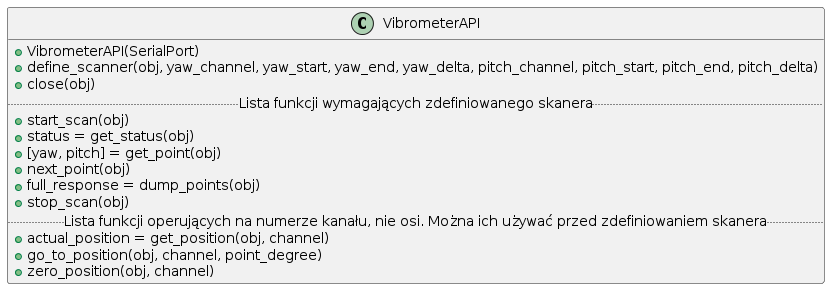
\includegraphics[width=\textwidth]{img/MatlabAPI_UML.png}
\caption{Diagram UML klasy sterującej systemem do pozycjonowania wibrometru.}
\label{img:matlab_api_uml}
\end{figure}


% \ref{lst:matlab_api_list}.
% \begin{lstlisting}[caption={Lista funkcji zaimplementowanych w API Matalb-owym},label={lst:matlab_api_list},style=Matlab,numbers=none]
% % Konstruktor:
% VibrometerAPI(SerialPort)

% % Funkcja definiująca skaner:
% define_scanner(obj, yaw_channel, yaw_start, yaw_end, yaw_delta, pitch_channel, pitch_start, pitch_end, pitch_delta)

% % Lista funkcji wymagających zdefiniowanego skanera:

% % Start skanowania, przemieszczenie do punktu startowego:
% start_scan(obj)
% % Pobranie statusu skanera:
% status = get_status(obj)
% %Pobranie obecnego, faktycznego punktu:
% [yaw, pitch] = get_point(obj)
% % Przemieszczenie do kolejnego punktu (pod warunkiem znajdowania się w stanie WaitingForNextPoint)
% next_point(obj)
% % Pobranie wszystkich punktów od początku pomiaru lub ostatniego wywołania tej komenda. Również przenosi skaner ze stanu Finished w stan Ready:
% full_response = dump_points(obj)
% % Przedwczesne przerwanie pomiaru:
% stop_scan(obj)

% % Lista funkcji pomocniczych, operujących na numerze kanału, nie osi. Można ich używać przed zdefiniowaniem skanera:

% % Zebranie faktycznej pozycji jednego z kanałów:
% actual_position = get_position(obj, channel)

% % Przejście na konkretną pozycję jednego z kanałów:
% go_to_position(obj, channel, point_degree)

% % Wyzerowanie pozycji kanału (Ustawienie obecnej pozycji jaki pozycji 0):
% zero_position(obj, channel)

% % Funkcja zamykająca połączenie portu szeregowego:
% close(obj)

% \end{lstlisting}


\subsection{Aplikacja GUI}
\label{cha:gui_app}
Dodatkowo, aby ułatwić manualną interakcję ze stołem, powstała aplikacja desktopowa z GUI, pozwalająca manualnie wywołać wszystkie dostępne operacje. Została napisana w języku C\#, frameworku Avalonia UI. Avalonia to open-sourcowy zestaw bibliotek, pozwalający pisać aplikacje cross-platformowe w języku C\#. Wspiera wszystkie wiodące systemy operacyjne, jak Windows, MacOS, Linux, Android czy iOS, ale także platforma ta podbija bardziej niszowe systemy, jak Tizen OS. Dodatkowo, poza aplikacjami na te systemy operacyjne, można napisać w nim stronę internetową, która będzie działać w większości wiodących przeglądarek internetowych. A co więcej, istnieje możliwość zbudowania jednego projektu dla wszystkich tych systemów, który wydziela wspólną część logiki programu. Jedynie system prezentacji danych jest różny dla różnych platform. Daje to możliwość zaoszczędzenia setek godzin pracy nad bliźniaczymi aplikacjami na różne systemy operacyjne. \cite{avalonia}

Na potrzeby tego projektu został natomiast wykorzystany jedynie ułamek możliwości tej platformy - ponieważ w ramach pracy powstała jedynie aplikacja na komputery z systemem Windows 7 lub nowszym.

Avalonia wspiera dwa schematy programowania. \textbf{Code-behind}, opierający się na podziale aplikacji na warstwę opisującą wygląd aplikacji, tzw. front-end oraz warstwę zawierającą odwołania (\textbf{callbacki}) od front-endu oraz logikę programu, tzw. back-end \cite{avalonia_CB}, oraz \textit{ReactiveUI}, implementujący wzorzec MVVM (\textbf{Model-View/View Model}). \cite{avalonia_MVVM} Wzorzec MVVM wprowadza dodatkową warstwę aplikacji pomiędzy back-end a front-end. We wzorcu tym logika programu jest zupełnie oddzielona od front-endu. Front-end, tutaj zwany \textbf{View}, jest jedynie samym opisem wyglądu aplikacji. Warstwa środkowa, czyli \textbf{View Model}, zawiera wszystkie odwołania od przycisków, kod aktualizujący odpowiednie wyświetlane wartości itp., jakie są potrzebne aby front-end był w stanie wejść w interakcję z back-endem. Na samym dole znajduje się back-end, tutaj zwany \textbf{Model}, gdzie znajduje się logika programu, zupełnie niezależna od reszty programu. Podejście to jest przede wszystkim bardzo przydatne w przypadku pisania aplikacji, które mają być kompilowane na wiele różnych platform.\cite{MVVMvsCB} W tej pracy, pomimo stosunkowej prostoty aplikacji, zdecydowano się na podejście MVVM, ponieważ daje to lepsze możliwości potencjalnej rozbudowy aplikacji w przyszłości. 


Aplikacja "VibrometerHostApp.exe", w celu zapewnienia większego komfortu użytkownikowi, została podzielona na 4 podstawowe ekrany, zgodnie z pewnymi grupami operacji jakie mogą być wykonywane przez użytkowników w jednym czasie.

\subsubsection{Ekran łączenia}
Ekran łączenia pozwala na wybór portu szeregowego z listy rozwijanej oraz połączenie się z wibrometrem na tym porcie. Dodatkowo zaimplementowane jest zabezpieczenie, blokujące połączenie z portem, na który podpięte jest coś innego niż stół - podczas próby łączenia sprawdzane są funkcje dostępne w urządzeniu. Jeżeli różnią się od funkcji wymaganych przez aplikację desktopową - połączenie jest odrzucane a użytkownik widzi kod błędu. Wygląd ekranu przedstawiony jest na zrzucie ekranu \ref{img:vib_host1}. Widać na nim efekt próby połączenia z urządzeniem na porcie "COM1"\, które nie jest stołem do pozycjonowania wibrometru. Użytkownik został poinformowany o tym przez aplikację Hostapp oraz nie została wykonana żadna kolejna akcja.

\begin{figure}[h!] 
\centering 
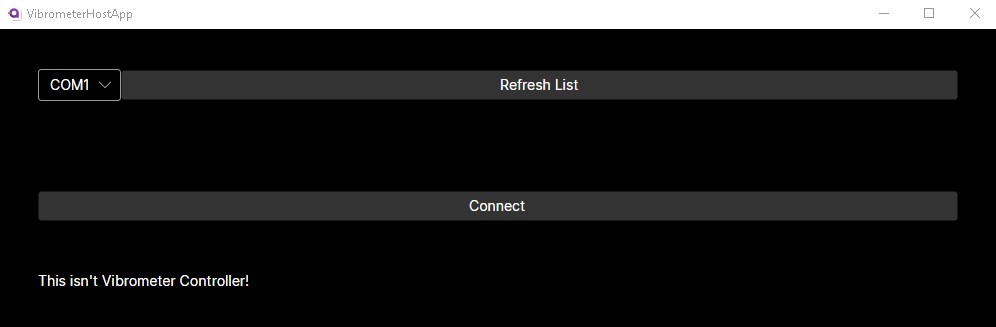
\includegraphics[width=\textwidth]{img/VibHost1.png}
\caption{Ekran łączności ze stołem do pozycjonowania.}
\label{img:vib_host1}
\end{figure}

\subsubsection{Ekran konfiguracyjny}
Kolejny jest ekran, pozwalający na konfigurację wibrometru - umożliwia on zdefiniowania 2 kanałów, yaw oraz pitch, w taki sam sposób jak definiowanie kanałów przy pomocy komend konsoli, lub API Matlab-owego. Po zdefiniowaniu obu kanałów można sprawdzić gotowość urządzenia i przejść do ekranu skanowania. W przypadku błędnej definicji kanałów, przycisk ready nie pozwoli przejść do kolejnego widoku. Wygląd ekranu przedstawiony jest na zrzucie ekranu \ref{img:vib_host2}. Widać na nim zdefiniowaną oś Yaw, wraz z pozytywną odpowiedzią od urządzenia, oraz jeszcze nie wypełnione wartości dla osi Pitch.

\begin{figure}[h!] 
\centering 
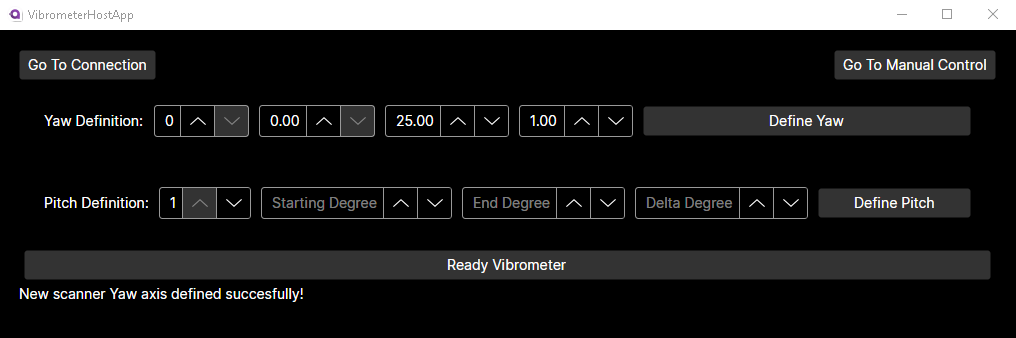
\includegraphics[width=\textwidth]{img/VibHost2.png}
\caption{Ekran konfiguracyjny stołu.}
\label{img:vib_host2}
\end{figure}

\subsubsection{Ekran skanowania}
Po udanym zdefiniowaniu osi skanowania wibrometru otwiera się ekran, dający możliwość kontroli nad samym procesem skanowania. Widać na nim takie przyciski, jak Start skanowania, Stop skanowania, zbieranie obecnego punktu, przemieszczanie się do kolejnego punktu, odczyt statusu oraz zrzut wszystkich odwiedzonych punktów. Przyciski te wykonują odpowiadające im komendy z konsoli, które opisane są rozdziale \ref{cha:commands}. Wygląd ekranu przedstawiony jest na zrzucie ekranu \ref{img:vib_host3}. Widać na nim skaner, który został przez użytkownika już uruchomiony, ponieważ zgłasza swój status jako WaitingForContinuation. Dodatkowo widać, że znajduje się na pozycji $1.35^{\circ}; 0.04^{\circ}$

\begin{figure}[h!] 
\centering 
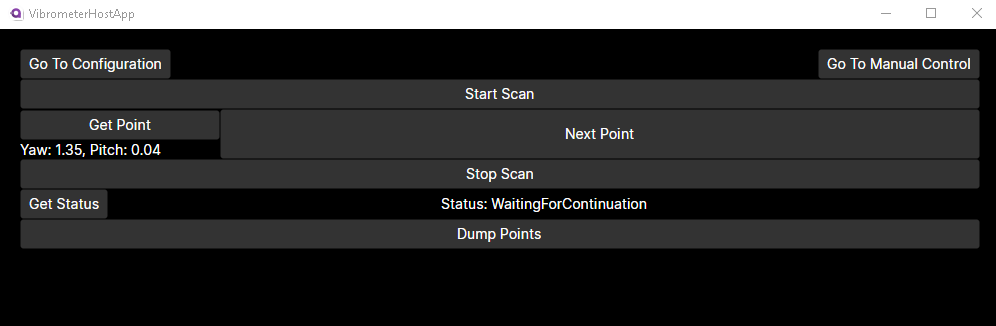
\includegraphics[width=\textwidth]{img/VibHost3.png}
\caption{Ekran skanowania.}
\label{img:vib_host3}
\end{figure}

\subsubsection{Ekran kontroli manualnej}
Podobnie jak w przypadku poprzednich form zarządzania urządzeniem, tutaj także jest dostęp do funkcjonalności zależnych jedynie od kanału, nie od zdefiniowanego skanera. Jednakże tutaj kontrola jest trochę większa niż w przypadku Matlaba - GUI daje dostęp do startowania i zatrzymywania silnika, oraz wysyłania silnika na konkretny kąt, wraz z odczytem obecnego kąta. Dodatkowo istnieje  możliwość wyzerowania pozycji - ustawienia obecnej pozycji jako kąt zerowy. Wygląd ekranu przedstawiony jest na zrzucie ekranu \ref{img:vib_host4}. Przedstawia on silnik na kanale 0 włączony i ustawiony na pozycji $10^{\circ}$. Natomiast silnik na kanale 1 jest wyłączony. Na przedstawionym zrzucie ekranu wyraźnie widać nieidealną precyzję kontroli pozycji - silnik został wysłany na kąt $10^{\circ}$, natomiast algorytm doprowadził go do pozycji $10.04^{\circ}$. 

\begin{figure}[h!] 
\centering 
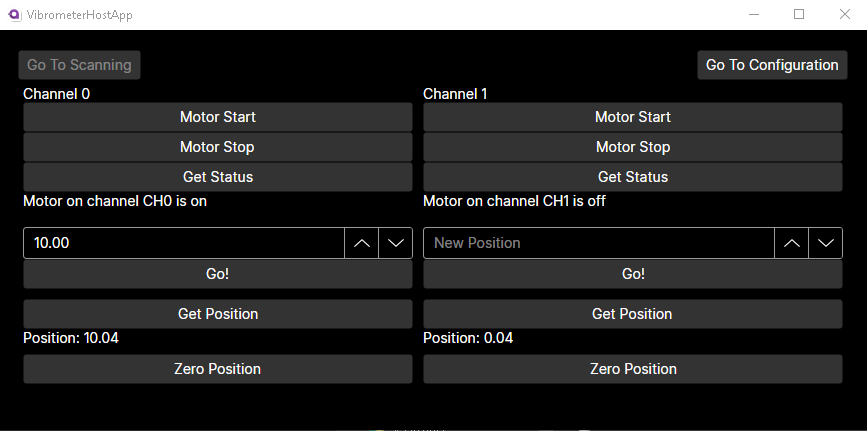
\includegraphics[width=\textwidth]{img/VibHost4.png}
\caption{Ekran kontroli manualnej.}
\label{img:vib_host4}
\end{figure}

Należy także wspomnieć o przyciskach do przechodzenia między ekranami. Każdy ekran zawiera dwa przyciski, w lewym i prawym górnym rogu. Pozwalają one na cofnięcie się do poprzednich ekranów, lub przejście do innego ekranu, który może być w danym momencie użytkownikowi potrzebny. W przypadku tego ekranu jest zaimplementowana blokada - nie da się przejść na ekran skanowania, jeżeli skaner nie jest zdefiniowany. Jest ona widoczna na zrzucie ekranu \ref{img:vib_host4}.
